\section{Experiments}
\label{sec:experiment}


\subsection{Eywabench: A Scalable Multi-task Multi-domain Scientific Benchmark}

Current scientific benchmarks are often limited to a narrow task family \cite{DBLP:journals/corr/WuRFGGPLP17, DBLP:journals/corr/abs-2502-14739}, a single domain \cite{DBLP:conf/emnlp/DaiYSZGHLZTGH25, DBLP:conf/emnlp/DaiYSZGHLZTGH25, DBLP:journals/corr/abs-2504-16074}, or one data format \cite{DBLP:journals/corr/abs-2505-19501, DBLP:journals/corr/abs-2507-03578, DBLP:conf/nips/JohnsonFGMBSF23, DBLP:conf/cvpr/0004WGWWCML0Z0025}, and therefore may not fully reflect the capability requirements of scientific agentic systems.
More specifically, two important scientific modalities, time series and tabular data, are often ignored or poorly evaluated in existing benchmarks.
To provide a holistic evaluation of agentic systems in scientific settings, we introduce \textit{Eywabench}, a scalable benchmark for multi-task and multi-domain scientific reasoning across heterogeneous modalities.
\textit{Eywabench} is constructed from a collection of datasets, including but not limited to DeepPrinciple \cite{song2025evaluating}, MMLU-Pro \cite{wang2024mmlu}, fev-bench \cite{DBLP:journals/corr/abs-2509-26468}, and TabArena \cite{DBLP:journals/corr/abs-2506-16791}.

\textbf{Multi-task and multi-domain coverage.} \textit{Eywabench} includes tasks spanning natural language, time series, and tabular data. The samples are organized into three domains: physical science, life science, and social science.
Each domain further contains three sub-domains: physical science includes material, energy, and space; life science includes biology, clinic, and drug; social science includes economy, business, and infrastructure.
Details of domains and sub-domains are provided in Appendix \ref{sec:dataset_details}.

\textbf{Scalability.} \textit{Eywabench} scales along both task volume and domain coverage.
Task volume can be increased by sampling new temporal windows, variables, and contextual combinations from source datasets.
Domain coverage can be expanded by applying the same construction pipeline to new time-series and tabular resources beyond fev-bench and TabArena. Moreover, the same design principle naturally extends to other scientific modalities (e.g., vision and geospatial earth observation) by incorporating corresponding datasets and specialist foundation models.

\begin{table}[!t]
    \centering
    \renewcommand{\arraystretch}{1.25}
    \caption{Overall performance comparison across scientific domains on \textit{EywaBench}. We compare all methods on three dimensions, including utility $(\uparrow)$, inference time $(\downarrow)$, and token consumption $(\downarrow)$. Best results are highlighted in bold and second-best results are underlined. Our proposed methods, EywaAgent, EywaMAS, and EywaOrchestra, achieve strong overall performance while maintaining competitive efficiency.}
    % \vspace{-8pt}
    \label{tab:main_comparison_eywabench}
    \small
    \resizebox{\textwidth}{!}{
    \begin{tabular}{l|c|ccc|ccc|ccc|c}
        \toprule
        \multirow{2}{*}{\textbf{Method}} &
        \multirow{2}{*}{\textbf{Metrics}} &
        \multicolumn{3}{c}{\textbf{Physical Science}} &
        \multicolumn{3}{c}{\textbf{Life Science}} &
        \multicolumn{3}{c}{\textbf{Social Science}}
        \\
        \cmidrule(lr){3-5}\cmidrule(lr){6-8}\cmidrule(lr){9-11}\cmidrule(lr){12-12}
        & & Material & Energy & Space & Biology & Clinic & Drug & Economy & Business & Infrastructure & Overall\\
        \midrule[-0.4ex]\midrule\addlinespace[-0.000ex]
        \rowcolor{gray!16}
        \multicolumn{12}{c}{
            \rule{0pt}{1.1em}
            \textbf{\textit{Single-Agent Setting}}
            \rule[-0.3em]{0pt}{1.1em}
        } \\
        [-0.4ex]\midrule\addlinespace[-0.000ex]

        \cellcolor{red!7}
        & Utility ($\uparrow$) & 0.5616 & 0.8202 & 0.5235 & 0.3402 & 0.4582 & 0.6004 & 0.7689 & 0.6528 & 0.6758 & 0.6154\\
        \cellcolor{red!7}\textbf{Single-LLM-Agent}
        & Time ($\downarrow$)  & 34.48 & 27.01 & 26.00 & 34.68 & 22.37 & 21.13 & 22.67 & 22.28 & 18.42 & 25.22\\
        \cellcolor{red!7}
        & Tokens ($\downarrow$) & 6367 & 4854 & 4512 & 6164 & 3618 & 3571 & 4097 & 3915 & 3327 & 4469\\
        [-0.4ex]\midrule\addlinespace[-0.000ex]
        
        \cellcolor{orange!7}
        & Utility ($\uparrow$)   & 0.5871 & 0.8390 & 0.6123 & 0.3718 & 0.5085 & 0.6199 & \textbf{0.8048} & \underline{0.7371} & 0.7060 & 0.6558\\
        \cellcolor{orange!7}\textbf{EywaAgent(Ours)}
        & Time ($\downarrow$)  & 34.88 & 24.42 & 23.12 & 30.84 & 20.32 & 15.84 & 19.71 & 20.98 & 15.99 & 22.78\\
                 
        \cellcolor{orange!7}
        & Tokens ($\downarrow$) & 5040 & 3167 & 3329 & 4858 & 2333 & 2210 & 2791 & 2444 & 2248 & 3137\\

        \addlinespace[-0.4ex] \midrule \addlinespace[-0.000ex]
        \rowcolor{gray!16}
        \multicolumn{12}{c}{
            \rule{0pt}{1.1em}
            \textbf{\textit{Multi-Agent Setting}}
            \rule[-0.3em]{0pt}{1.1em}
        } \\
        [-0.4ex]\midrule\addlinespace[-0.000ex]

        \cellcolor{yellow!7}
        & Utility ($\uparrow$)   & 0.5687 & 0.8667 & 0.6244 & 0.3623 & 0.4504 & 0.6215 & 0.7523 & 0.6880 & 0.6362 & 0.6294\\
        \cellcolor{yellow!7}\textbf{Refine MAS \citeyearpar{DBLP:conf/nips/MadaanTGHGW0DPY23}}
        & Time ($\downarrow$)  & 72.76 & 64.22 & 79.65 & 75.21 & 51.89 & 50.63 & 62.33 & 48.54 & 47.49 & 60.59\\
        \cellcolor{yellow!7}
        & Tokens ($\downarrow$) & 11013 & 9009 & 10043 & 10497 & 7029 & 7498 & 8924 & 6997 & 7438 & 8673\\
        [-0.4ex]\midrule\addlinespace[-0.000ex]

        \cellcolor{green!7}
        & Utility ($\uparrow$)   & 0.5602 & 0.8656 & 0.6543 & 0.3438 & 0.4738 & 0.6198 & 0.7729 & 0.6907 & 0.7237 & 0.6460\\
        \cellcolor{green!7}\textbf{Debate MAS \citeyearpar{DBLP:conf/icml/Du00TM24}}
        & Time ($\downarrow$)  & 82.06 & 79.46 & 74.75 & 101.64 & 78.19 & 63.98 & 92.72 & 72.46 & 60.73 & 78.22\\
        \cellcolor{green!7}
        & Tokens ($\downarrow$) & 16652 & 14278 & 13614 & 17007 & 11159 & 10447 & 14694 & 10953 & 10311 & 13216\\
        [-0.4ex]\midrule\addlinespace[-0.000ex]

        \cellcolor{teal!7}
        & Utility ($\uparrow$)   & 0.5909 & 0.8069 & 0.5863 & 0.3580 & 0.4722 & 0.5686 & 0.7499 & 0.7004 & 0.6938 & 0.6273\\
        \cellcolor{teal!7}\textbf{MoA \citeyearpar{DBLP:conf/iclr/WangWAZZ25}}
        & Time ($\downarrow$)  & 90.15 & 56.95 & 69.32 & 59.10 & 46.53 & 44.31 & 57.35 & 48.29 & 47.34 & 57.75\\
        \cellcolor{teal!7}
        & Tokens ($\downarrow$) & 25327 & 16453 & 17332 & 15980 & 11014 & 10344 & 16114 & 11690 & 12365 & 15317\\
        [-0.4ex]\midrule\addlinespace[-0.000ex]

        \cellcolor{blue!7}
        & Utility ($\uparrow$)   & 0.5831 & 0.8057 & 0.5723 & \underline{0.3737} & 0.4490 & 0.6211 & 0.6923 & 0.6390 & 0.7180 & 0.6188\\
        \cellcolor{blue!7}\textbf{X-MAS \citeyearpar{DBLP:journals/corr/abs-2505-16997}}
        & Time ($\downarrow$)  & 104.48 & 86.63 & 79.06 & 88.20 & 67.94 & 59.76 & 75.50 & 72.82 & 62.95 & 77.42\\
        \cellcolor{blue!7}
        & Tokens ($\downarrow$) & 24149 & 19808 & 16584 & 18451 & 12549 & 11907 & 16499 & 14007 & 14056 & 16537\\
        [-0.4ex]\bottomrule

        \cellcolor{violet!7}
        & Utility ($\uparrow$)   & \textbf{0.6381} & \textbf{0.8742} & \underline{0.6899} & \textbf{0.3798} & \underline{0.5086} & \underline{0.6248} & \underline{0.7959} & 0.7284 & \textbf{0.7406} & \textbf{0.6761}\\
        \cellcolor{violet!7}\textbf{EywaMAS (Ours)}
        & Time ($\downarrow$)  & 77.25 & 75.96 & 72.51 & 111.92 & 59.97 & 59.23 & 68.40 & 58.11 & 46.49 & 72.11\\
        \cellcolor{violet!7}
        & Tokens ($\downarrow$) & 14529 & 11709 & 11787 & 16502 & 9407 & 8078 & 11044 & 9470 & 8912 & 11214\\
        
        \addlinespace[-0.4ex] \midrule \addlinespace[-0.000ex]
        \rowcolor{gray!16}
        \multicolumn{12}{c}{
            \rule{0pt}{1.1em}
            \textbf{\textit{Dynamic Orchestration}}
            \rule[-0.3em]{0pt}{1.1em}
        } \\
        [-0.4ex]\midrule\addlinespace[-0.000ex]

        \cellcolor{pink!7}
            & Utility ($\uparrow$)   & \underline{0.6249} & \underline{0.8711} & \textbf{0.7187} & 0.3682 & \textbf{0.5159} & \textbf{0.6319} & 0.7830 & \textbf{0.7388} & \underline{0.7298} & \underline{0.6746}\\
        \cellcolor{pink!7}\textbf{EywaOrchestra (Ours)}
            & Time ($\downarrow$)  & 61.78 & 39.92 & 75.47 & 67.88 & 45.38 & 45.94 & 49.13 & 34.18 & 28.80 & 48.16\\
        \cellcolor{pink!7}
            & Tokens ($\downarrow$) & 11535 & 7723 & 10810 & 11315 & 7050 & 6495 & 7117 & 7264 & 6892 & 8335\\
        [-0.4ex]\bottomrule\addlinespace[-0.000ex]

    \end{tabular}
    }
    % \vspace{-4pt}
\end{table}


\textbf{Evaluation metric.} \textit{Eywabench} uses a unified utility score $u \in [0,1]$ across all tasks, so results from different modalities are directly comparable.
For natural-language-centered tasks, utility is computed with a soft-match score between predictions and references; for time-series and tabular tasks, utility is derived from normalized prediction errors.
The benchmark reports per-domain mean utility and also mean utility over all tasks. Detailed metric definitions are provided in the Appendix \ref{sec:dataset_details}.

\subsection{Experimental Setup}
\textbf{Language models and foundation models.} We use gpt-5-nano as the default language model and we also evaluate other models from and beyond the GPT family in our later experiments.
We have two foundation models to build EywaAgents. Chronos \cite{DBLP:journals/tmlr/AnsariSTZMSSRPK24, DBLP:journals/corr/abs-2510-15821} is a general-purpose foundation model for time series. 
TabPFN \cite{DBLP:conf/iclr/Hollmann0EH23} is a transformer-based foundation model that uses in-context-learning to solve tabular prediction problems in a forward pass.
Neither foundation models provide a native language interface.


\textbf{Baseline methods.} We compare \textit{Eywa} against three baseline groups: (a) \emph{single-agent LLM baselines} built on the same backbone, including GPT \cite{DBLP:journals/corr/abs-2601-03267}, Gemini \cite{team2023gemini, comanici2025gemini}, and Claude \cite{claude} families of models; (b) \emph{homogeneous LLM-based multi-agent baselines}, including Refine \cite{DBLP:conf/nips/MadaanTGHGW0DPY23} and Debate \cite{DBLP:conf/icml/Du00TM24}, instantiated with the same backbone model; (c) \emph{heterogeneous LLM-based multi-agent baselines}, including Mixture-of-Agents (MoA) \cite{DBLP:conf/iclr/WangWAZZ25} and X-MAS \cite{DBLP:journals/corr/abs-2505-16997}, which combine multiple heterogeneous language models.


\textbf{Implementation details.} We implement \textit{Tsaheylu} (FM-LLM interface) using LangChain agents and FastMCP servers.
Each foundation model is deployed as an independent MCP backend, served over streamable HTTP on a local port.
Each \textit{EywaAgent} connects a language model to its designated MCP endpoint, loads task data into server-side storage, and invokes the foundation model on demand.
All methods are allowed up to two retries when their outputs cannot be parsed. In practice, Eywa rarely triggers this fallback because specialized foundation models already produce structured outputs in one shot, whereas LLM-only baselines benefit more from retries.
For all runs, we record wall-clock latency and token usage. The results are averaged over multiple runs on a 13th Gen Intel(R) Core(TM) i9-13900H CPU with 64GB RAM. 

\subsection{Main Results}

\begin{wrapfigure}{r}{0.45\textwidth}
  \begin{center}
  \vspace{-10pt}
    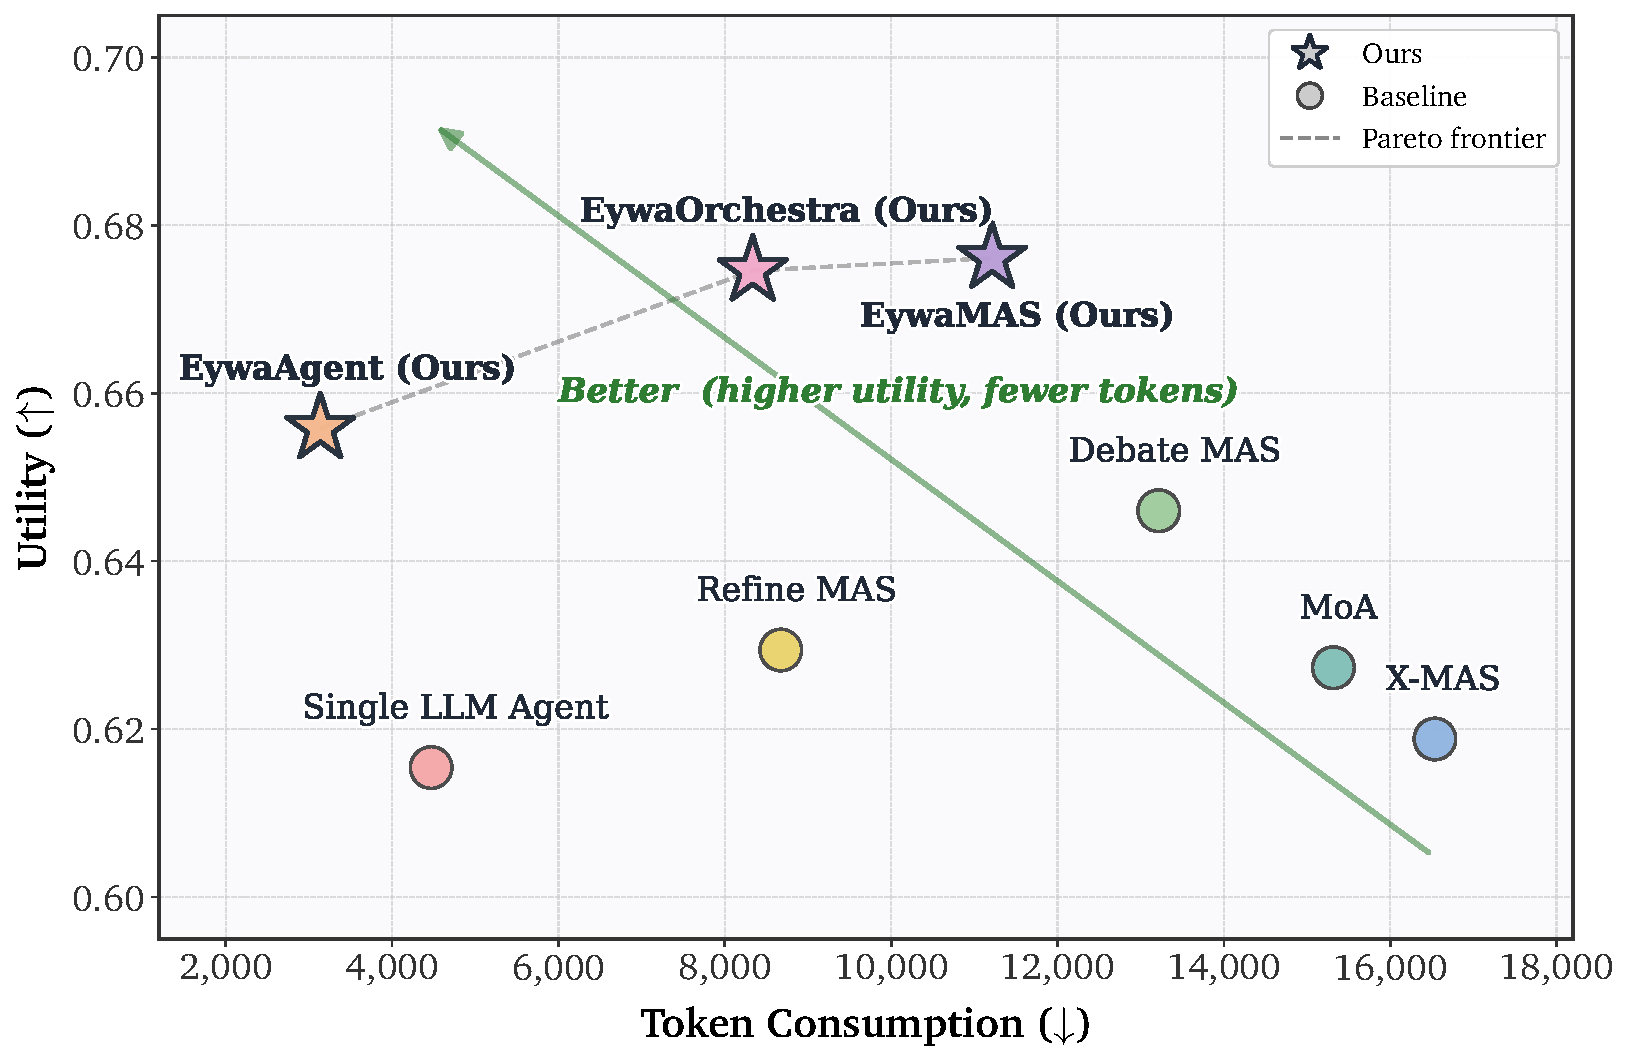
\includegraphics[width=0.45\textwidth]{figures/utility_token_tradeoff.pdf}
  \end{center}
  \vspace{-16pt}
  \caption{Overall utility and token consumption of different methods. Full results in Figure \ref{fig:tradeoff_per_domain}. 
  }
  \vspace{-14pt}
\end{wrapfigure}

We evaluate all methods on \textit{Eywabench} under a unified protocol.
For \textit{EywaAgent} and \textit{EywaMAS}, which do not perform dynamic orchestration, we assign the foundation model for each sample using expert-defined configurations. \textit{EywaMAS} uses debate topology by default.
For \textit{EywaOrchestra}, the conductor automatically selects the foundation model and topology conditioned on the sample.

Table \ref{tab:main_comparison_eywabench} reports the performance of all methods on \textit{Eywabench} in scientific settings. We highlight the following observations: (a) \textit{EywaAgent} improves both quality and efficiency under the same backbone.
Compared with the corresponding single-agent baseline, \textit{EywaAgent} increases average utility by $6.6\%$, while reducing latency and cutting token usage by nearly $30\%$ through delegation to domain-specific foundation models.
(b) \textit{EywaMAS} outperforms homogeneous MAS baselines in scientific settings.
\textit{EywaMAS} achieves the best overall utility and outperforms homogeneous multi-agent baselines. Compared with \textit{Refine}, \textit{EywaMAS} delivers significantly stronger utility. Compared with \textit{Debate}, \textit{EywaMAS} not only achieves better utility but also requires fewer tokens under the same debate topology.
(c) {LLM-only heterogeneity is insufficient for scientific tasks.} Heterogeneous LLM-only MAS methods do not consistently outperform strong homogeneous MAS baselines on \textit{Eywabench}. This suggests that, for scientific workloads, cross-modality heterogeneity is more critical than only combining heterogeneous language models.
(d) {Not every domain benefits equally from heavier multi-agent computation.} In domains such as economy and business, single-agent \textit{EywaAgent} is already highly competitive, indicating that always using complex multi-agent topologies is not necessarily optimal. This observation motivates adaptive orchestration conditioned on task and domain characteristics.
(e) \textit{EywaOrchestra} approaches EywaMAS with lower cost and automation. \textit{EywaOrchestra} uses no expert configuration and instead lets the conductor automatically construct the system for each sample. Despite this, \textit{EywaOrchestra} reaches utility close to expert-designed \textit{EywaMAS}, and even surpasses it on several sub-domains. At the same time, dynamic orchestration substantially reduces inference cost in both latency and token usage compared to fixed multi-agent systems.

\subsection{Further Analysis}



\begin{figure*}[t]
  \begin{subfigure}[t]{0.32\linewidth}
    \centering
    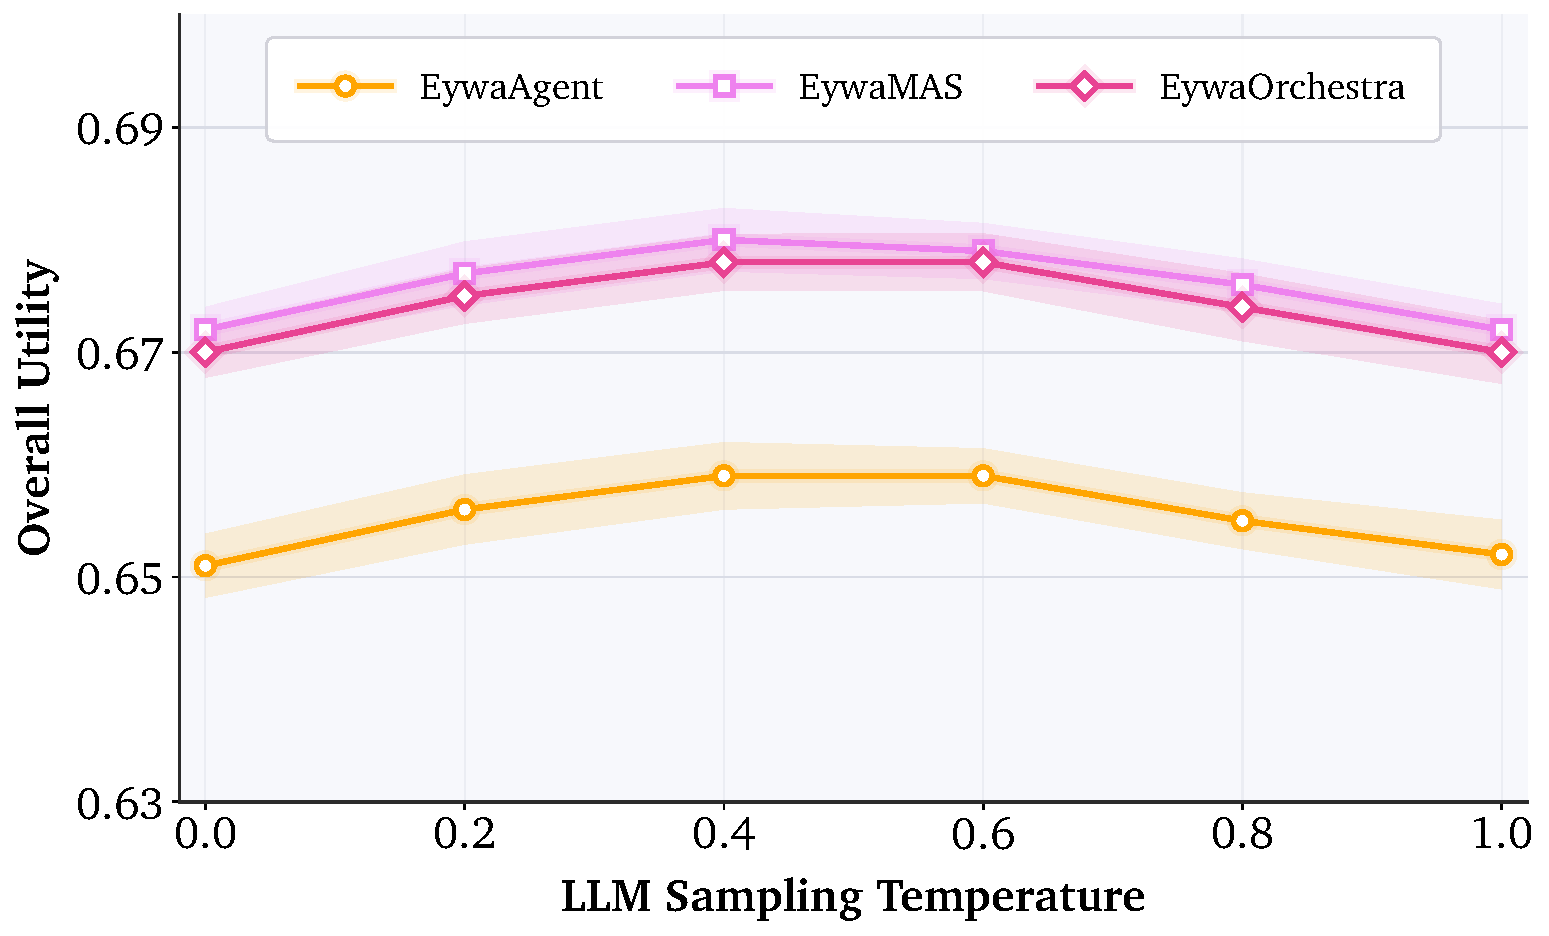
\includegraphics[width=\linewidth]{figures/hyperparameter/hyperparameter_temperature_study.pdf}
    \caption{LLM Temperature Ablation.}
  \end{subfigure}\hfill
  \begin{subfigure}[t]{0.32\linewidth}
    \centering
    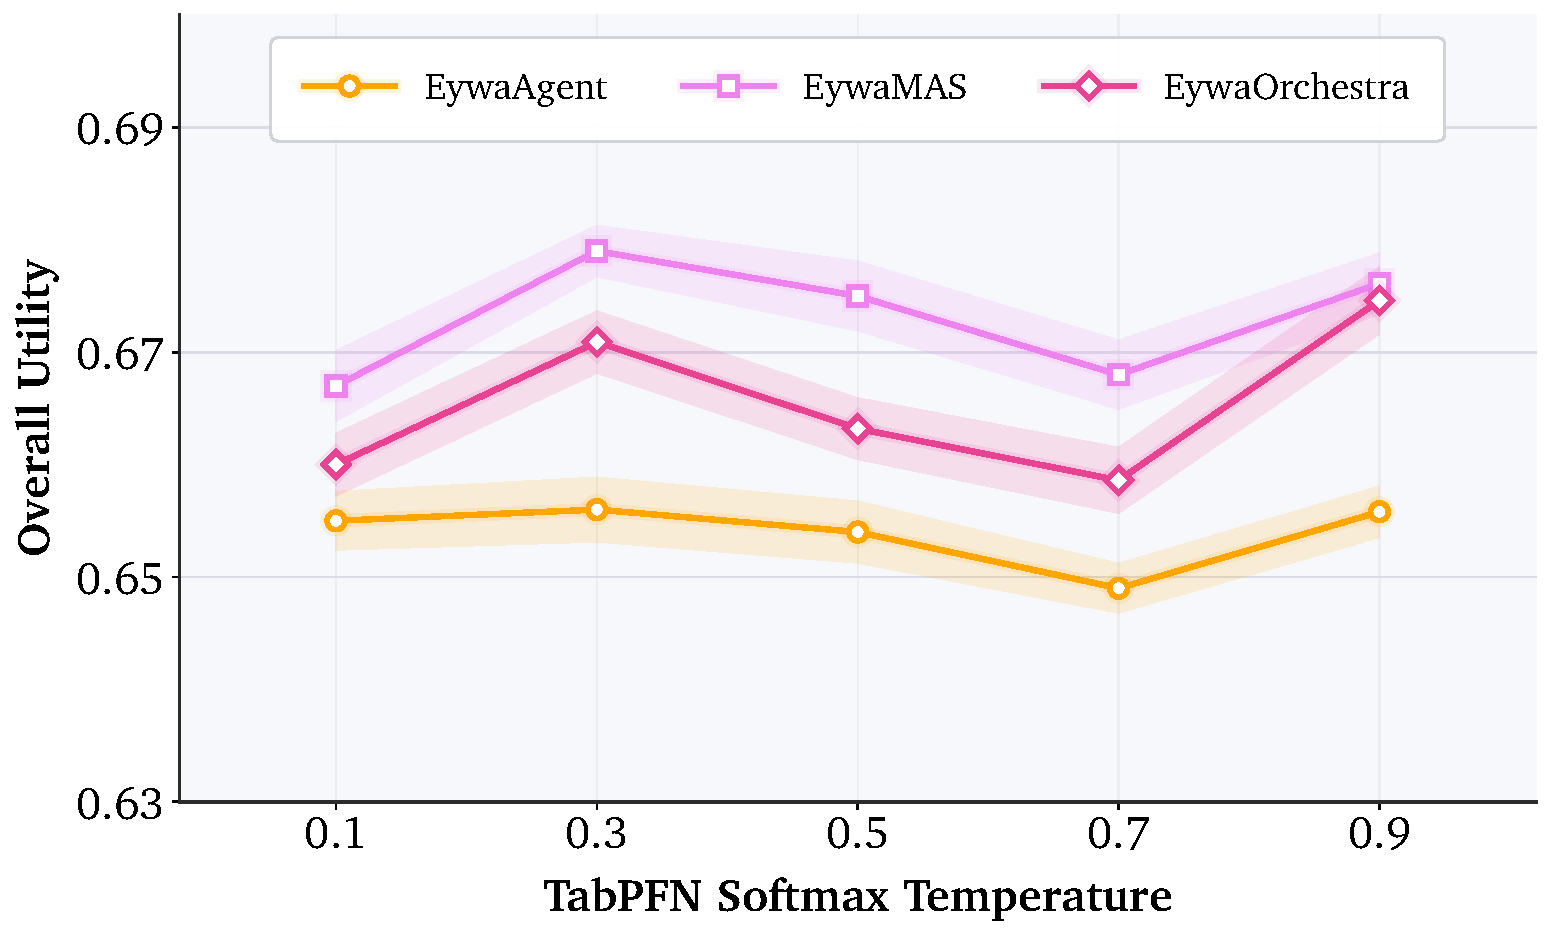
\includegraphics[width=\linewidth]{figures/hyperparameter/hyperparameter_temperature_study_fm.pdf}
    \caption{FM Temperature Ablation.}
  \end{subfigure}\hfill
  \begin{subfigure}[t]{0.32\linewidth}
    \centering
    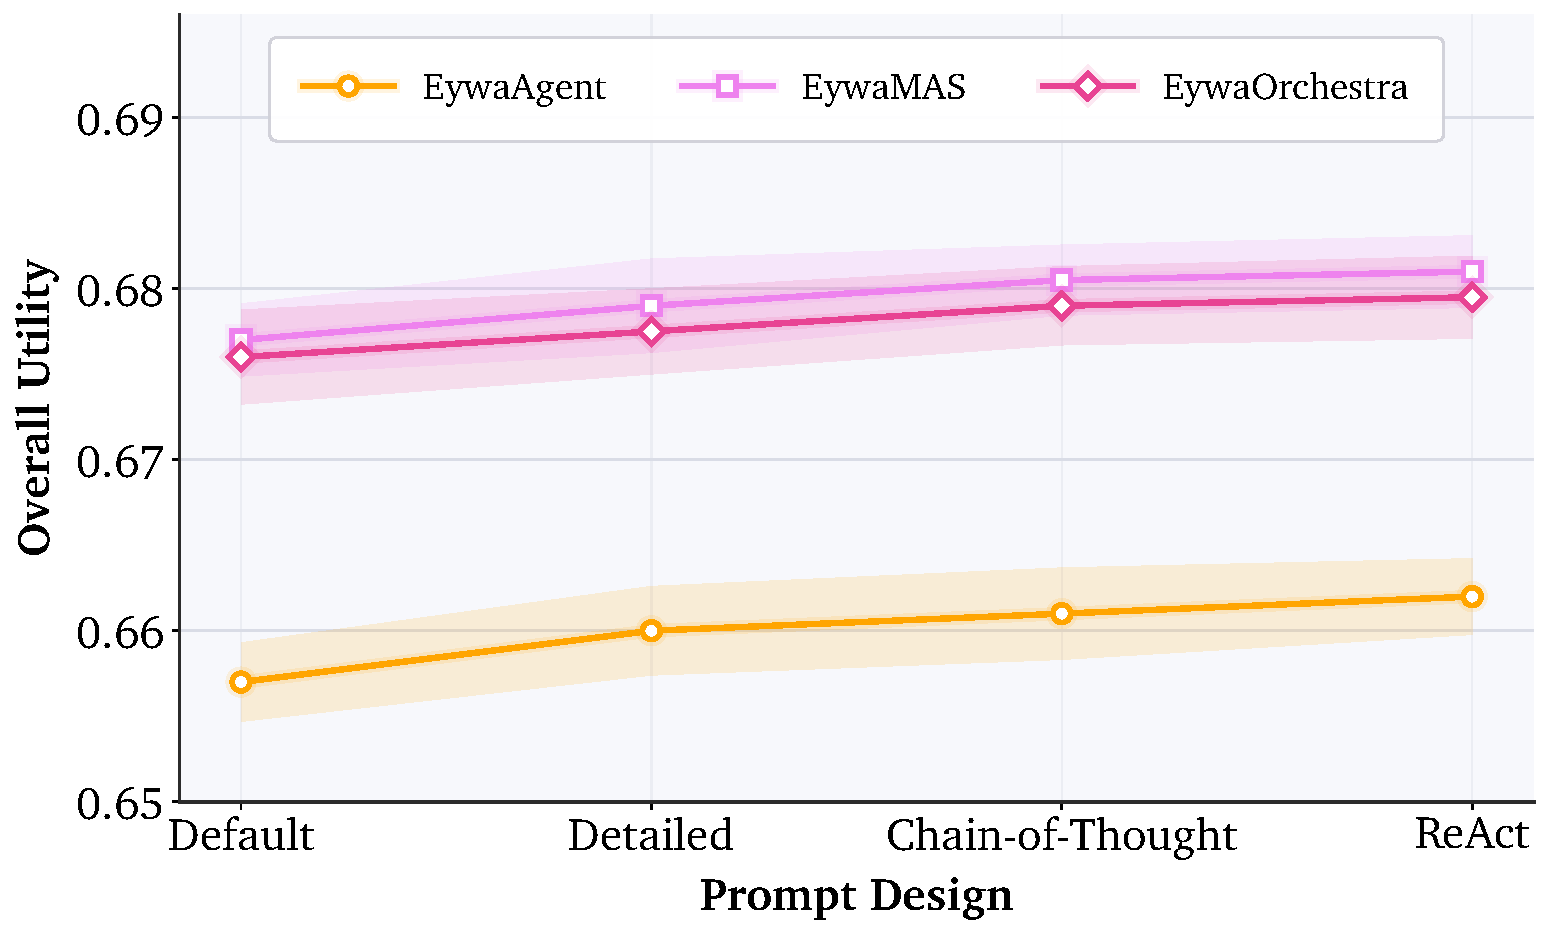
\includegraphics[width=\linewidth]{figures/hyperparameter/hyperparameter_prompt_sensitivity_study.pdf}
    \caption{Prompt Design Ablation.}
  \end{subfigure}\\[4pt]

\caption{Hyperparameter sensitivity analysis of \textit{Eywa}. We evaluate \textit{EywaAgent}, \textit{EywaMAS}, and \textit{EywaOrchestra} under different ablation configurations. \textbf{(a)} LLM temperature ablation: \textit{Eywa} maintains stable performance across varying LLM sampling temperatures. \textbf{(b)} FM temperature ablation: \textit{Eywa} remains robust under different TabPFN softmax temperatures. \textbf{(c)} Prompt design ablation: \textit{Eywa} remains effective across different prompting strategies, and generally benefits from more structured prompt designs. Overall, the results demonstrate that \textit{Eywa} is compatible and robust to a broad range of design choices.}
\label{fig:hyperparameter_sensitivity}
\vspace{-3mm}
\end{figure*}



\textbf{Hyperparameter sensitivity.} We perform hyperparameter studies of both language models and foundation models to evaluate the robustness of \textit{Eywa}. Specifically, we vary the LLM sampling temperature, the foundation model temperature in TabPFN, and the prompt design used by the language-model interface. As shown in Figure~\ref{fig:hyperparameter_sensitivity}, \textit{Eywa} remains stable across a broad range of configurations. In particular, the performance of \textit{EywaAgent}, \textit{EywaMAS}, and \textit{EywaOrchestra} stays robust as the LLM sampling temperature varies, while consistently peaking around a moderate temperature. Ablation on varying the TabPFN softmax temperature also suggests that the benefit of integrating domain-specific foundation models is robust to foundation-model calibration. We further compare several prompt designs. The \textit{Detailed} prompt provides more comprehensive task descriptions and general guidance, \textit{Chain-of-Thought} \cite{DBLP:conf/nips/Wei0SBIXCLZ22} encourages the model to reason step by step, and \textit{ReAct} \cite{DBLP:conf/iclr/YaoZYDSN023} further interleaves reasoning with actions, enabling the model to decide more explicitly when to invoke tools or domain-specific foundation models during problem solving. While \textit{Eywa} performs well under all prompting strategies, more structured prompts generally lead to slightly better utility. Overall, these results demonstrate that the gains of \textit{Eywa} are not tied to a particular hyperparameter choice or prompt template. Additional ablation studies such as turn ablation are provided in Appendix~\ref{ap:more_ablation}.



\renewcommand{\arraystretch}{1.00}
\begin{wraptable}{r}{0.45\linewidth}
    \centering
    \caption{Ablation results of \textit{EywaAgent} with different LLM backends. \textit{Eywa} benefits from more powerful LLMs to achieve better performance.}
    % \vspace{-8pt}
    \label{tab:model_ablation_compact}
    \resizebox{0.45\textwidth}{!}{
    \begin{tabular}{l|c|cccc}
        \toprule
        \textbf{Method} & \textbf{Metrics} & \textbf{Physical} & \textbf{Life} & \textbf{Social} & \textbf{Overall}\\
        \midrule[-0.4ex]\midrule\addlinespace[-0.000ex]

        \multirow{3}{*}{\makecell{gpt-4.1-nano}}
        & Utility ($\uparrow$) & 0.6547 & 0.4010 & 0.6269 & 0.5680\\
        & Time ($\downarrow$)  & 14.25 & 28.66 & 16.89 & 19.61\\
        & Tokens ($\downarrow$) & 1314 & 927 & 1160 & 1139\\
        [-0.4ex]\midrule\addlinespace[-0.000ex]

        \multirow{3}{*}{\makecell{gpt-5-nano}}
        & Utility ($\uparrow$) & 0.6914 & 0.5001 & 0.7488 & 0.6558\\
        & Time ($\downarrow$)  & 28.04 & 22.33 & 18.71 & 22.78\\
        & Tokens ($\downarrow$) & 3907 & 3134 & 2491 & 3137\\
        [-0.4ex]\midrule\addlinespace[-0.000ex]

        \multirow{3}{*}{\makecell{gpt-5-mini}}
        & Utility ($\uparrow$) & 0.7191 & 0.5035 & 0.7444 & 0.6640\\
        & Time ($\downarrow$)  & 23.18 & 30.70 & 18.51 & 23.63\\
        & Tokens ($\downarrow$) & 2875 & 2617 & 1949 & 2444\\
        [-0.4ex]\bottomrule
    \end{tabular}
    }
    \vspace{-6pt}
\end{wraptable}



\textbf{Ablation on \textit{Eywa} with different LLM backends.} 
To evaluate the impact of LLM backbone choice, we instantiate \textit{EywaAgent} with three backends: gpt-4.1-nano, gpt-5-nano, and gpt-5-mini.
As shown in Table \ref{tab:model_ablation_compact}, \textit{Eywa} remains consistently effective across physical, life, and social science domains under all three backbones.
We also observe a clear upward trend in overall utility as backend capability increases, indicating that \textit{Eywa} is robust to backbone selection while still benefiting from stronger LLM priors.
Complete backbone ablations for \textit{EywaMAS} and \textit{EywaOrchestra} are reported in Appendix Table \ref{tab:ablation_backend_llm}.
A systematic investigation of scaling behavior and cost-performance trade-offs across LLM backbones remains important future work.



\textbf{Case study.} We provide qualitative case studies to further illustrate how \textit{Eywa} coordinates language models and domain-specific foundation models. Case Study A compares a language-only LLM agent with \textit{EywaAgent} on the same task over structured financial signals. Case Study B further illustrates the role of \textit{EywaOrchestra}. Due to space limit, detailed examples and analyses are deferred to Appendix~\ref{ap:case_study}.